% !TEX root = ../master-thesis.tex











% \newpage

% \begin{figure}[h]
%     \centering
%     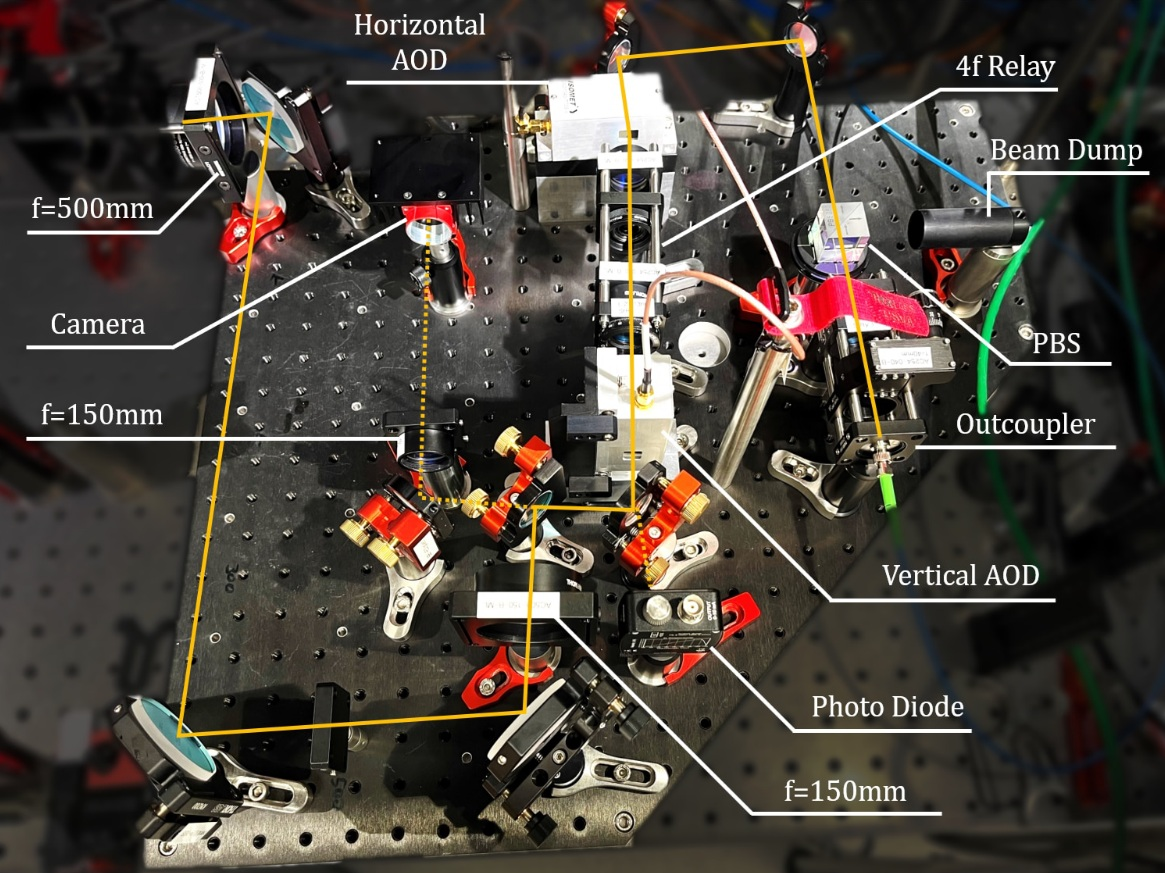
\includegraphics[width=0.5\textwidth]{imgs/tw-setup.jpg}
%     \caption{
%     \textbf{Optical setup for 2D tweezer array.} 
%     The beam path (solid orange line) includes two orthogonal AODs, a $4f$ relay, and diagnostic components. Dashed lines indicate monitoring light paths. Taken from \cite{culemann_construction_2024}.
%     }
%     \label{fig:tw-setup}
% \end{figure}


 












% \begin{figure}
%     \centering
%     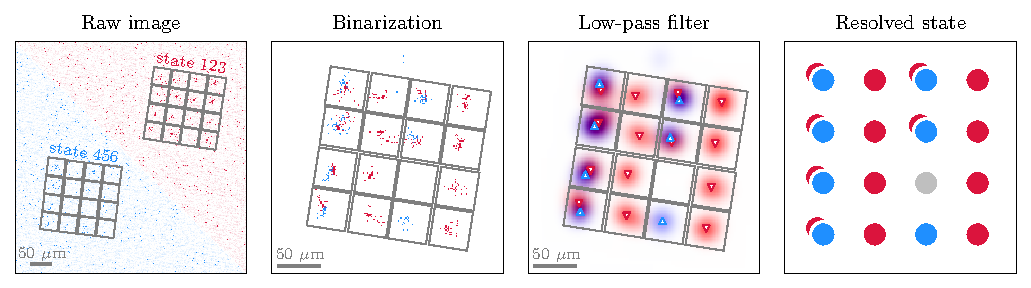
\includegraphics{fig-py/imaging-spin-resolved.pdf}
%     \caption{
%         \textbf{Spin-resolved single-atom imaging.}
%         Spatially separated $\sigma_+$ and $\sigma_-$ fluorescence is imaged onto two distinct regions of the camera. The binarization step identifies photon counts above a threshold, followed by a low-pass filter to extract spatially localized signals. Final spin states are assigned based on relative signal strength in each channel:
%         \raisebox{-1pt}{\scalebox{1.5}{\textcolor{ublue}{\textbullet}}} -- $\ket{1}$, 
%         \raisebox{-1pt}{\scalebox{1.5}{\textcolor{ured}{\textbullet}}} -- $\ket{2}$, 
%         \raisebox{-1pt}{\scalebox{1.5}{\textcolor{uhole}{\textbullet}}} -- no atom.
%     }
%     \label{fig:spin-resolved}
% \end{figure}


% Lorem ipsum dolor sit amet, consectetur adipisicing elit, sed do eiusmod
% tempor incididunt ut labore et dolore magna aliqua. Ut enim ad minim veniam,
% quis nostrud exercitation ullamco laboris nisi ut aliquip ex ea commodo
% consequat. Duis aute irure dolor in reprehenderit in voluptate velit esse
% cillum dolore eu fugiat nulla pariatur. Excepteur sint occaecat cupidatat non
% proident, sunt in culpa qui officia deserunt mollit anim id est laborum.


% \newline
% \phantom{42}
% \newline
% \addletter{100}{c} \phantom{4}
% 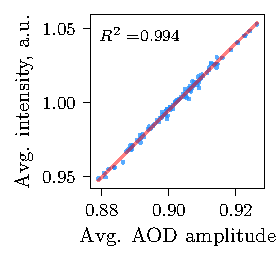
\includegraphics{fig-py/crosstalk-camera-amp.pdf}
% \phantom{4}
% \addletter{100}{d} \phantom{4}
% 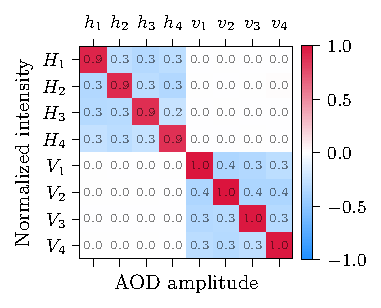
\includegraphics{fig-py/crosstalk-camera.pdf}
% \hfill
% \phantom{4}

